\documentclass[11pt]{article}

\usepackage[most]{tcolorbox}
\usepackage{times}
\usepackage{epsf}
\usepackage{epsfig}
\usepackage{amsmath, alltt, amssymb, xspace}
\usepackage{wrapfig}
\usepackage{fancyhdr}
\usepackage{url}
\usepackage{verbatim}
\usepackage{fancyvrb}
\usepackage{adjustbox}
\usepackage{listings}
\usepackage{color}
\usepackage{subfigure}
\usepackage{cite}
\usepackage{sidecap}
\usepackage{pifont}
\usepackage{mdframed}
\usepackage{textcomp}
\usepackage{enumitem}


% Horizontal alignment
\topmargin      -0.50in  % distance to headers
\oddsidemargin  0.0in
\evensidemargin 0.0in
\textwidth      6.5in
\textheight     8.9in 

\newcommand{\todo}[1]{
\vspace{0.1in}
\fbox{\parbox{6in}{TODO: #1}}
\vspace{0.1in}
}


\newcommand{\unix}{{\tt Unix}\xspace}
\newcommand{\linux}{{\tt Linux}\xspace}
\newcommand{\minix}{{\tt Minix}\xspace}
\newcommand{\ubuntu}{{\tt Ubuntu}\xspace}
\newcommand{\setuid}{{\tt Set-UID}\xspace}
\newcommand{\openssl} {\texttt{openssl}}


\pagestyle{fancy}
\lhead{\bfseries SEED Labs}
\chead{}
\rhead{\small \thepage}
\lfoot{}
\cfoot{}
\rfoot{}


\definecolor{dkgreen}{rgb}{0,0.6,0}
\definecolor{gray}{rgb}{0.5,0.5,0.5}
\definecolor{mauve}{rgb}{0.58,0,0.82}
\definecolor{lightgray}{gray}{0.90}


\lstset{%
  frame=none,
  language=,
  backgroundcolor=\color{lightgray},
  aboveskip=3mm,
  belowskip=3mm,
  showstringspaces=false,
%  columns=flexible,
  basicstyle={\small\ttfamily},
  numbers=none,
  numberstyle=\tiny\color{gray},
  keywordstyle=\color{blue},
  commentstyle=\color{dkgreen},
  stringstyle=\color{mauve},
  breaklines=true,
  breakatwhitespace=true,
  tabsize=3,
  columns=fullflexible,
  keepspaces=true,
  escapeinside={(*@}{@*)}
}

\newcommand{\newnote}[1]{
\vspace{0.1in}
\noindent
\fbox{\parbox{1.0\textwidth}{\textbf{Note:} #1}}
%\vspace{0.1in}
}


%% Submission
\newcommand{\seedsubmission}{You need to submit a detailed lab report, with screenshots,
to describe what you have done and what you have observed.
You also need to provide explanation
to the observations that are interesting or surprising.
Please also list the important code snippets followed by
explanation. Simply attaching code without any explanation will not
receive credits.}

%% Book
\newcommand{\seedbook}{\textit{Computer \& Internet Security: A Hands-on Approach}, 2nd
Edition, by Wenliang Du. See details at \url{https://www.handsonsecurity.net}.}

%% Videos
\newcommand{\seedisvideo}{\textit{Internet Security: A Hands-on Approach},
by Wenliang Du. See details at \url{https://www.handsonsecurity.net/video.html}.}

\newcommand{\seedcsvideo}{\textit{Computer Security: A Hands-on Approach},
by Wenliang Du. See details at \url{https://www.handsonsecurity.net/video.html}.}

%% Lab Environment
\newcommand{\seedenvironment}{This lab has been tested on our pre-built
Ubuntu 16.04 VM, which can be downloaded from the SEED website. }

\newcommand{\seedenvironmentA}{This lab has been tested on our pre-built
Ubuntu 16.04 VM, which can be downloaded from the SEED website. }

\newcommand{\seedenvironmentB}{This lab has been tested on our pre-built
Ubuntu 20.04 VM, which can be downloaded from the SEED website. }

\newcommand{\seedenvironmentAB}{This lab has been tested on our pre-built
Ubuntu 16.04 and 20.04 VMs, which can be downloaded from the SEED website. }

\newcommand{\nodependency}{Since we use containers to set up the lab environment, 
this lab does not depend too much on our SEED VM. You can do this lab
using other VMs or physical machines. }







\newcommand{\seedlabcopyright}[1]{
\vspace{0.1in}
\fbox{\parbox{6in}{\small Copyright \copyright\ {#1}\ \ by Wenliang Du.\\
      This work is licensed under a Creative Commons
      Attribution-NonCommercial-ShareAlike 4.0 International License.
      If you remix, transform, or build upon the material, 
      this copyright notice must be left intact, or reproduced in a way that is reasonable to
      the medium in which the work is being re-published.}}
\vspace{0.1in}
}





\newcommand{\rootingFigs}{./Figs}

\lhead{\bfseries SEED Labs -- Android Device Rooting Lab}

\begin{document}


\begin{center}
{\LARGE Android Device Rooting Lab}
\end{center}

\seedlabcopyright{2018}



% *******************************************
% SECTION
% ******************************************* 
\section{Overview}

Android devices do not allow their owners to have the root privilege on the
device. This is fine for normal customers, but for users who want to make
deep customizations on their devices, this is too restrictive. There are
ways to overcome these restrictions, most of which require the root
privilege on the device. The process of gaining the root device on Android
devices is called \textit{rooting}. Being able to root Android devices is a
very useful skill for security experts. 


The objective of this lab is two-fold. First, through this lab, students
will get familiar with the process of device rooting and understand why
certain steps are needed. Many people can root Android devices, but not
many people fully understand why things have to be done in a particular
way. Second, the entire rooting mechanism involves
many pieces of knowledge about the Android system and operating system in
general, so it serves as a great vehicle for students to gain such in-depth
system knowledge. In this lab, we will ask students to develop a complete rooting
package from scratch, and demonstrate how to use the package to root the
Android VM provided by us. 


\section{Background Knowledge}


\subsection{Background Knowledge about Rooting}

The purpose of rooting an Android device is to gain the root privilege
inside the Android OS. There are many reasons why people want to do that.
For example, Android devices often come with many pre-installed system apps that are
useless most of the time, but they take storage space, RAM,
system resources, and drain device battery. These useless
apps are generally known as bloatware; they are installed
in protected places, and only the root user (or other privileged user) 
can remove them. Although the device is owned by a user,
the user is not allowed to run code using the root privilege. 
Users can only get the root privilege if the device is rooted. 
In general, rooting allows users to customize their phones, removing restrictions,
adding new features, and making changes to the system. There are several
approaches to root an Android device, and we will discuss them in more
details in this lab. Figure~\ref{fig:rooting:androidrooting} provides a summary of these
approaches.


\paragraph{Modifying Android from inside.}
The first rooting approach is doing it from inside Android. For an un-rooted device, everything that
the user runs is running with a normal user ID (not root). Therefore,
rooting from inside Android means that the user has to gain the root
privilege as a normal user. Obviously, this is impossible for 
a perfectly implemented operating system. However, the chances are that
Android may not be perfectly implemented, so there might exist
vulnerabilities in the system. If these vulnerabilities are inside the kernel or daemons 
running with the root privilege, users can exploit these vulnerabilities to
gain the root privilege. This is one of the techniques to root Android
devices. 

In the past, there were many rooting exploits, such as
\texttt{RageAgainstTheCage}, which took advantage of 
\texttt{RLIMIT\_NPROC} max, the value specifying how many processes a given UID can run. 
This exploit first uses \texttt{"adb  shell"} to run a 
shell on the device via the \texttt{adb} daemon. The UID of the shell will
be 2000. The exploit then forks new processes until the number of processes
have reached the limit and the fork call will fail. 
At this point, the exploit kills the \texttt{adbd} daemon, and then
reconnect to it using \texttt{"adb shell"}. This causes the system to  
restart the \texttt{adb} daemon. When \texttt{adb} is started, it always
has the root privilege, but it will drop the privilege to UID 2000 using   
\texttt{setuid(2000)}. Unfortunately, the UID 2000 has already used up its 
process quota, so the call will fail. Unfortunately, the \texttt{adb}
daemon fails to handle the failure correctly: instead of exiting, it keeps
running, while retaining the root privilege. As results, the 
\texttt{"adb shell"} command will give users a root shell. 
This vulnerability has already been fixed after Android 2.2. 



\begin{figure}[htb]
	\begin{center}
		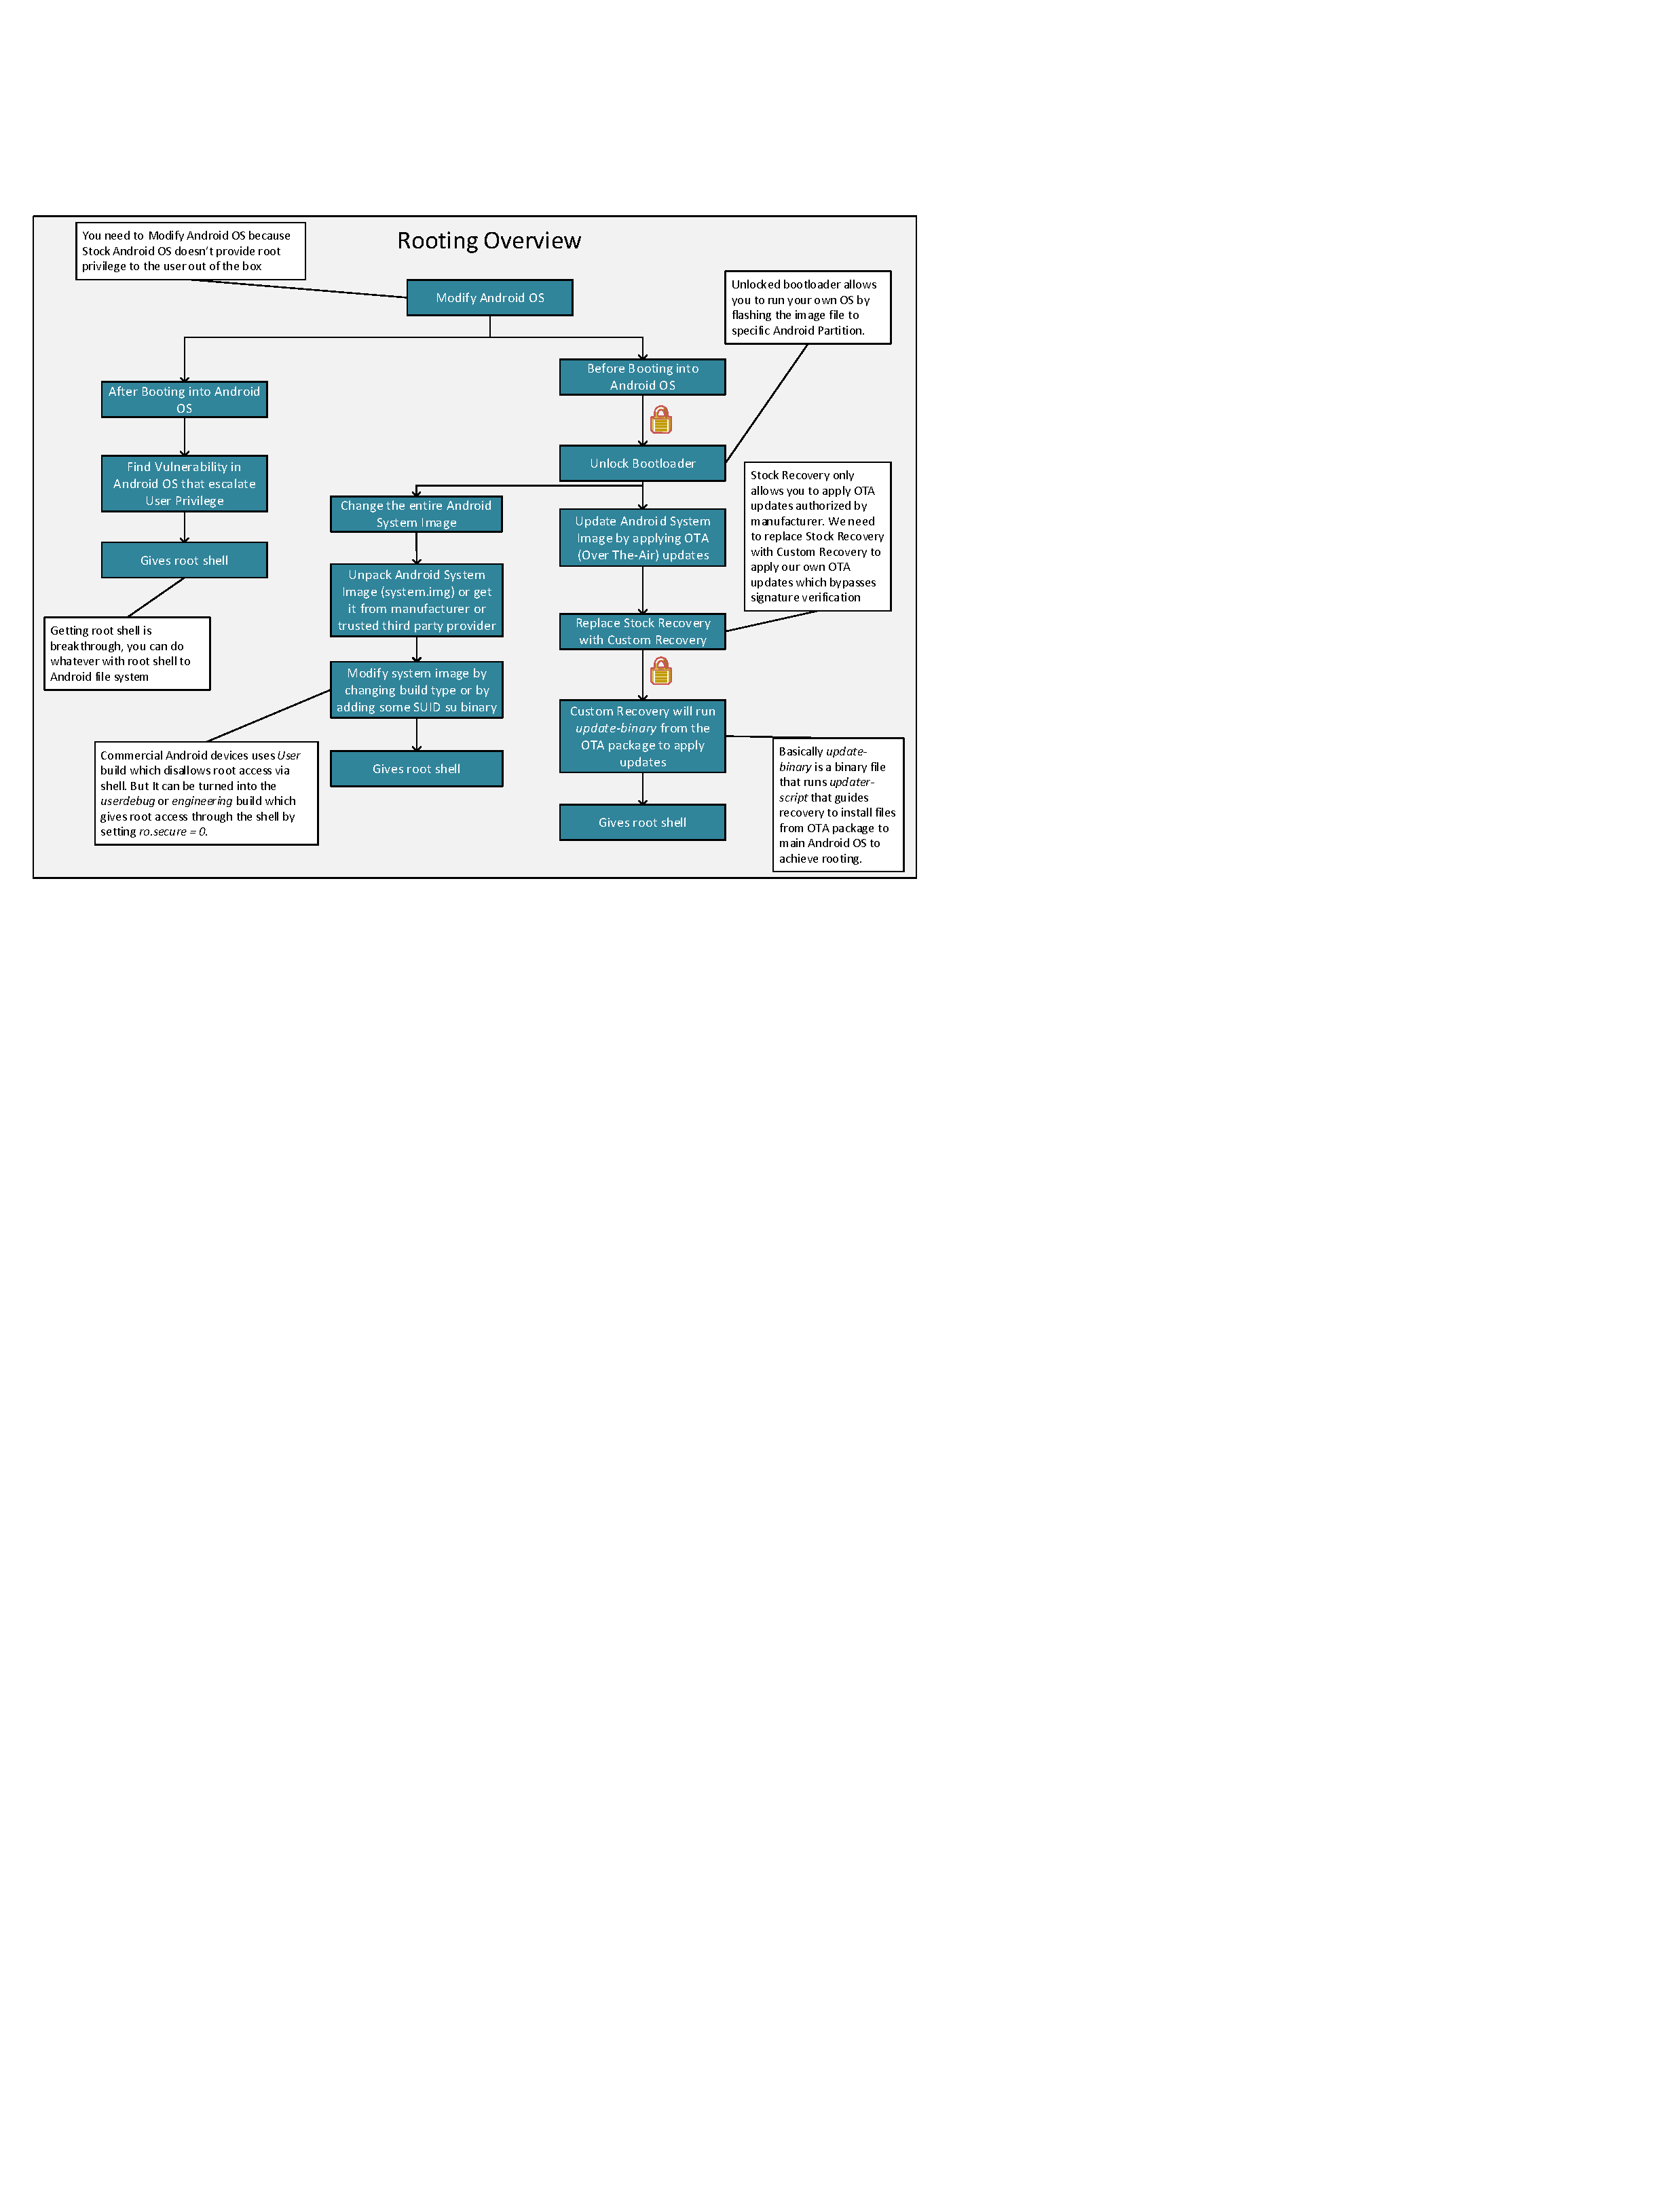
\includegraphics[width=1.0\textwidth]{\rootingFigs/AndroidRooting.pdf}
	\end{center}
	\caption{Rooting Android Devices}
	\label{fig:rooting:androidrooting}
\end{figure}
 

\paragraph{Modifying Android from outside.}
Since Android's access control prevents a normal user from modifying the
part of the system that is only modifiable by the root, doing 
it inside Android is going to subject to the access control. However, if we can
do it from outside, we are not subject to Android's access control any
more. This leads to the second approach, which is to directly modify 
Android's system files from outside. 

 
Assume that another operating system is installed on your Android device. 
This means that the device has a dual-boot configuration, allowing you to boot into any
of these two operating systems when the device powers on. If we boot into
this second operating system, and become the root for this OS, 
we can mount the partition used by the
Android system. Once this partition is mounted, we can access all the files
stored inside the partition. Because Android is not running, its access
control has no use. Therefore, we can make arbitrary changes to its files.
For example, we can place some programs in the system, and modify Android's
initialization scripts, and ask Android to run our programs as a root
during its initialization process. 


The good news is that most Android devices do have the second operating
system installed, and it is called \textit{recovery OS}. As the name
indicates, it is meant for recovery purposes, but it is mostly used for
updating operating system. The bad news is that this operating system also
has access controls, preventing users from running arbitrary programs or
commands. Recovery OS is typically placed on devices by vendors, who use 
the OS to update Android, but not wanting users to make arbitrary updates. 
To enforce that, recovery OSes do not give users a shell prompt, preventing
users from running arbitrary commands. Instead, they take a package provided
from outside (either from users or downloaded from the Internet); the
package contains the commands and files needed for updating the 
Android OS. This mechanism is widely
used for OS update, and it is called Over-The-Air (OTA) update. The package is
called OTA package, which has a standard file structure that we will
talk about later. 


Most recovery OSes only accept the packages made by the vendors to ensure
that any update to the Android OS is approved by the vendors. This is enforced
using digital signatures, i.e., the package needs to be signed by vendors,
or it will not be accepted by the recovery OS. This protection becomes a
roadblock for rooting, because the package that we use for rooting purposes
will not come from the vendor of the device. We need to find ways to bypass
this access control. 



\paragraph{Reinstall recovery OS.}
Instead of bypassing the access controls of the recovery OS, the easiest
way is to replace the entire stock recovery OS with another recovery OS
that does not have such access controls. This new recovery OS, called
custom recovery OS, will not include the signature
verification part, so we can provide any OTA packages to the recovery OS.
This will allow us to make arbitrary changes to the Android partition.

Here is another bad news. There is another access control that prevents us
from replacing the stock recovery OS, and this time it is the bootloader. 
Bootloader is a low level code that loads an operating system or some other
system software for the computer after the computer is powered on. When a
bootloader is ``locked'', it will simply load one of the OSes that is
already installed on the device, leaving no chances for users to modify any
of the pre-installed OSes. If a bootloader can be unlocked, it
will add another option, which allows users to install custom operating
systems on the device, as well as replacing the existing ones. The process
is often referred to as flashing custom OS. 

Manufacturers usually make their bootloaders locked out of
the box because they want to be in control of what software is running the
device. However, most manufacturers do provide ways for users to unlock the bootloader on their devices, 
provided that by doing so users will lose all of their data, as well as the warranties.  



\subsection{Background Knowledge about OTA}

OTA is a standard technique for devices to update Android operating systems. Since rooting
also needs to update Android OS, OTA becomes a popular choice. In this section, we will
describe the structure of the OTA package. Students need to build their own OTA package from
the scratch in this lab.


\begin{figure}[htb]
	\begin{center}
		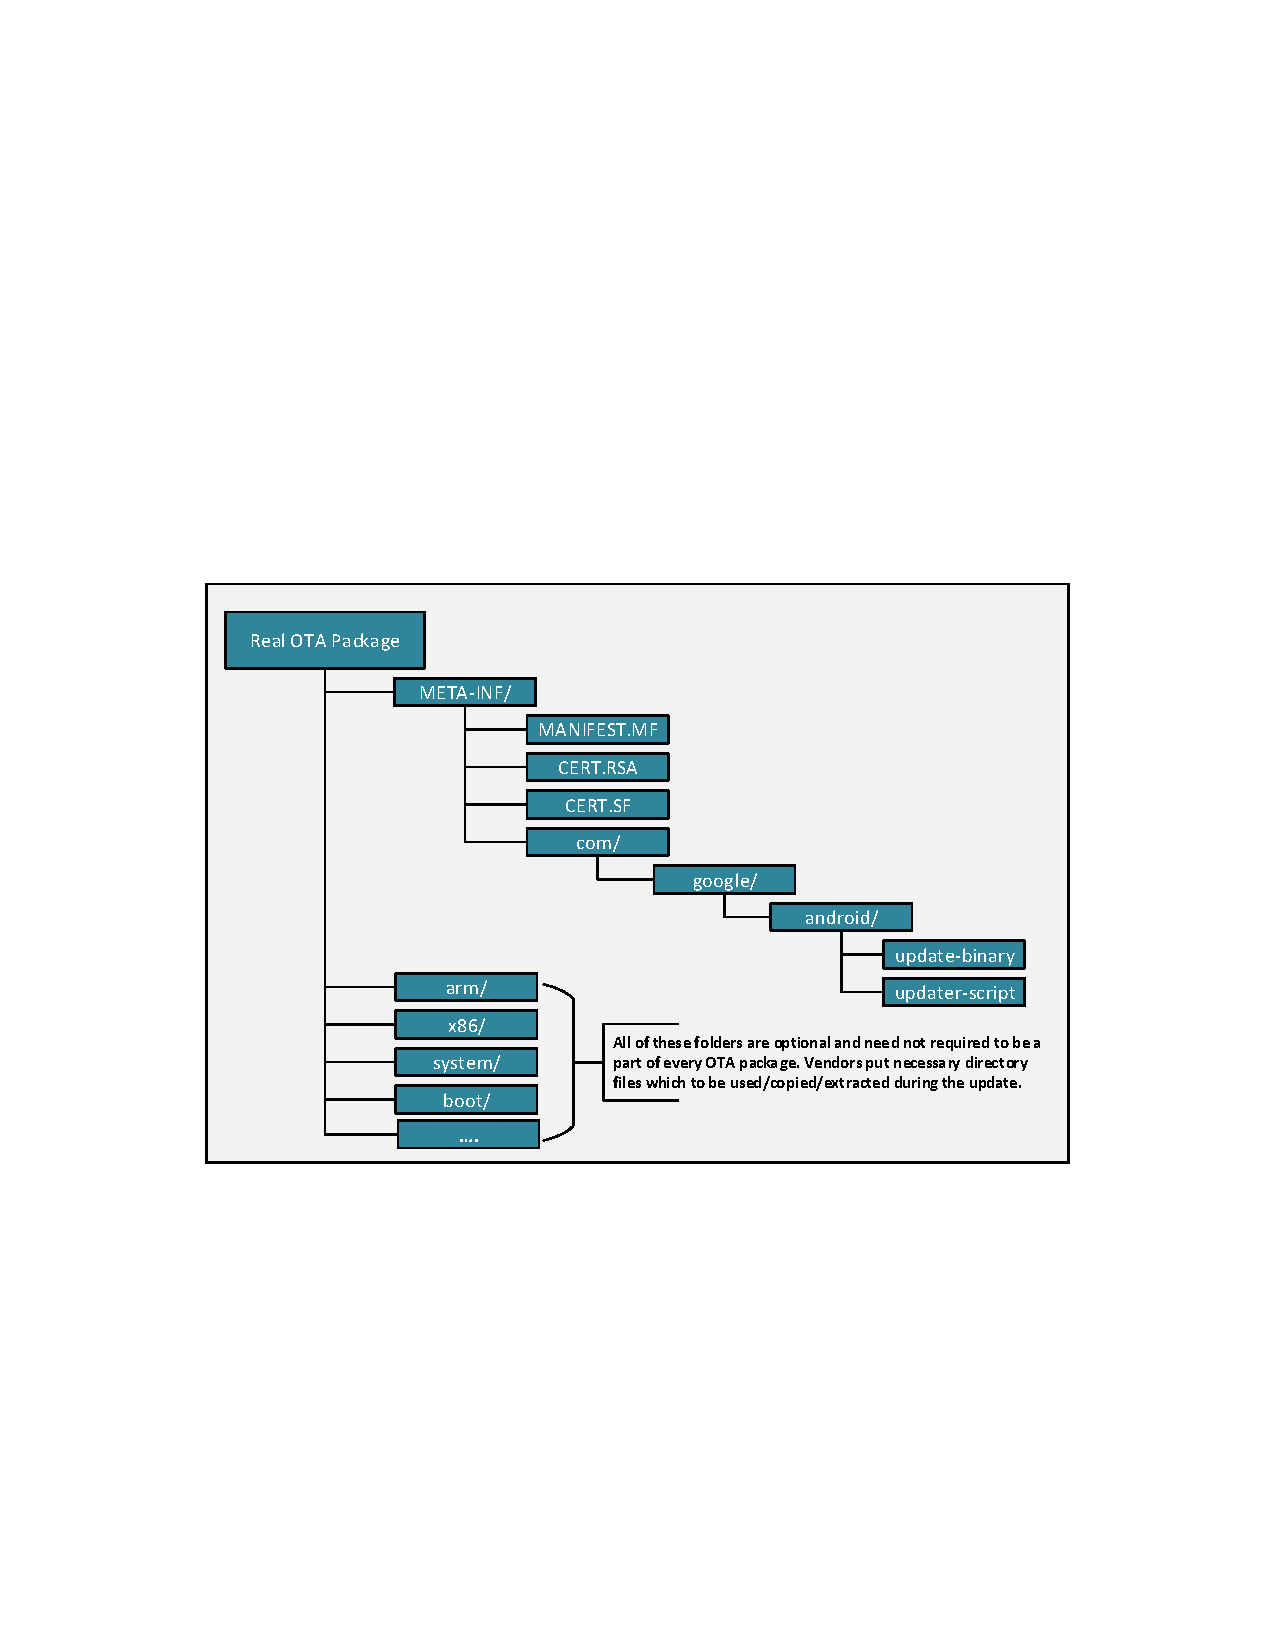
\includegraphics[width=0.8\textwidth]{\rootingFigs/Real_OTA.pdf}
	\end{center}
	\caption{OTA Structure}
	\label{fig:rooting:real_OTA}
\end{figure}
 

OTA package is just a zip file and its structure is depicted in 
Figure~\ref{fig:rooting:real_OTA}. Of particular interest to this lab is the 
\texttt{META-INF} folder, which includes signature and certificates of the package along with
two very important files named \texttt{update-binary} and \texttt{updater-script}.

\begin{itemize} 
\item \texttt{META-INF/com/google/android/update-binary}: This binary is executed
by the recovery OS to apply OTA updates; it loads and execute
\texttt{updater-script}.

\item \texttt{META-INF/com/google/android/updater-script}: This is an installation
script which is interpreted by \texttt{update-binary}. It is written using a script
language called \texttt{Edify}, which describes the required action to be performed
to apply updates. 

%Edify supports control structure such as if and else and
%also allows us to use built-in function to make logical decisions within
%the script. 
\end{itemize}

After signature verification on the OTA package, the recovery OS extracts
the \texttt{update-binary} executable from the OTA package to 
the \texttt{/tmp} directory and runs it by passing three arguments as follows:  

\begin{lstlisting}[frame=single, caption={}, label=label]
update-binary version output package
where, version is the version of recovery API,
       output is the command pipe that update-binary uses to  communicate 
                          with recovery,
       package is the path of the OTA package,


An Example would be:  update-binary 3 stdout /sdcard/ota.zip
\end{lstlisting}
 

On a successful execution of \texttt{updater-script}, the recovery OS copies the
execution logs to the \texttt{/cache/recovery/} directory and reboots into the Android
OS. Execution logs can be accessible from the Android OS after rebooting.
This is how android system is updated by using OTA package.


\section{Lab Environment}

In this lab, we assume that the bootloader on the device can be unlocked,
and the stock recovery OS can be replaced. Replacing the recovery OS in the VM environment
is quite difficult, and it is not within the scope of this lab. The Android
VM that you download from our web site already has a custom recovery OS
installed. Actually, we simply use Ubuntu 16.04 as
the ``recovery OS''. Technically, this is not a recovery OS; it is just another OS
installed on the device. We use this general-purpose OS to emulate what
users can do using a custom recovery OS. Once users boot into this OS, they can run any
arbitrary commands (as root), and be able to make arbitrary changes to the
Android partition. 



Students who have a physical Android device and want to know how to root a
real device, they can follow our guidelines in
Section~\ref{sec:rooting:guidelines}. However, other than the step to replace
the recovery OS, everything else is the same as what we do in this lab.  


Another important thing to know is that our Android VM is already rooted. That was
done when we built the VM from the Android source code. Our VM build is
actually a \textit{userdebug} build, and several doors were built into the VM
to allow root access.  We choose this build because several of our other labs require the root
access. Real Android devices use \textit{user} build, which do not have these doors
for root access. Details about these doors can be found in our VM manual. 
In this lab, students are not allowed to use those doors to gain the root
access; they have to use the OTA mechanism to achieve that.



\section{Lab Task 1: Build a simple OTA package}

In this lab, students will build a simple OTA package from scratch, and 
use it to root Android OS. We divide this complicated task into several
tasks, each focusing on a specific goal. Here are the goals that we would
like to achieve:

\begin{itemize} 
\item How to inject a program into the Android OS from the recovery OS?
\item How to get our injected program to run automatically, and with the root privilege?
\item How to write a program that can give us the root shell?
\end{itemize} 
  

In this Task 1, we focus on how to inject a program into the Android OS
from the recovery OS, and then get Android to run our injected program
using the root privilege. At this point, we are not focusing on the
actual thing that we can do in this program, as long as it is something that
requires the root privilege. For the sake of simplicity, let us simply
create a dummy file in the \texttt{/system} folder of Android, which
requires the root privilege (the \texttt{/system} folder is not 
writable by normal users). The following command puts a word
``hello'' in \texttt{/system/dummy} (we put this command in a shell script 
file called \texttt{dummy.sh}):  

\begin{lstlisting}
echo hello > /system/dummy
\end{lstlisting}

%\todo{We assume that the Android OS is mounted in the \texttt{/android} 
%directory of the recovery OS.}	


\paragraph{Step 1: Write the update script.}
The \texttt{update-binary} file in the OTA package is the executable file 
that will be first executed by the recovery OS. This is where we get the OS update started.
This file can be a binary executable, or just a simple script file. For the
latter case, the recovery OS should already have the binary executable
(e.g. \texttt{bash}) to execute the script file. In this task, we will
simply use a shell script, as our recover OS (\texttt{Ubuntu}) does have 
\texttt{bash} installed. 


Our purpose for \texttt{update-binary} is two-fold: (1) inject our \texttt{dummy.sh} program
into the Android OS, and (2) change the Android OS configuration file, so 
our \texttt{dummy.sh} can be automatically executed with the root privilege
when Android boots up. For the first task, students need to figure out
where to place \texttt{dummy.sh}, and how to set up its permissions. 
It should be noted that the file has to be placed into the Android
partition, which is already mounted to the \texttt{/android} directory in
the recovery OS. 


For the second purpose, we need to get \texttt{dummy.sh} to run
automatically when Android boots up, and we need to make sure that it runs
with the root privilege. There are many ways to achieve this. In this task,
we use one approach related to Linux, and in the next task, we will use a different
approach related to Android framework.

Android is built on top of the Linux operating system. When it boots
up, its underlying Linux boots up first, which conducts system
initialization, including starting essential daemon processes.  
The booting procedure, using the root privilege, runs a file called 
\texttt{/system/etc/init.sh}~\footnote{This is
for Android-x86 build; for the ARM build, the file name is different.} 
for part of the initialization. Therefore, if we can insert a command 
into \texttt{init.sh} file, we can run our \texttt{dummy.sh} file with the
root privilege. 

If we can do it manually, we can simply edit the \texttt{init.sh}, and add
a new command in it, but we are writing an OTA package, so the actions
to modify the file need to be coded in our \texttt{update-binary}
file. There are many ways to code that, and we will use the \texttt{sed}
command, which is stream editor for filtering and transforming text. 
Our idea is to find where the statement \texttt{"return 0"} is inside \texttt{init.sh},
and insert a command before that, essentially placing the command before 
the program in \texttt{init.sh} finishes.  

\begin{lstlisting}[frame=single, caption={}, label=label]
sed -i "/return 0/i /system/xbin/dummy.sh" /android/system/etc/init.sh

Explanation: 
  -  "-i": edit files in place.
  -  "/return 0/": match the line that has the content "return 0".
  -  "i": insert before the matching line.
  -  "/system/xbin/dummy.sh": the content to be inserted. We need to copy
        the dummy.sh file to the corresponding folder first.
  -  "/android/system/etc/init.sh": the target file modified by "sed".
\end{lstlisting}


\paragraph{Step 2: Build the OTA Package.}
Constructing an OTA package is quite straightforward. All we need to do is to put our files in
their corresponding folders according to Figure~\ref{fig:rooting:real_OTA}.
We need to maintain the same structure as what is shown in the figure, but 
you do not need to create all the files that are not needed for our 
task~(such as signature and optional files). 
You can put the \texttt{dummy.sh} file in any place of your 
OTA package, as long as the location matches with your command in 
the \texttt{update-binary}. After creating the file structure, we can use
the \texttt{zip} command to create a zip file:

\begin{lstlisting}
zip -r my_ota.zip ./
\end{lstlisting}

You should include the file structure of your OTA package in your report. You can 
run the \texttt{"unzip -l"} command to do that.



\paragraph{Step 3: Run the OTA Package}
After building the OTA package, we can provide it to the recovery OS, which
will run it automatically. However, that is how it works with a real
recovery OS. In our lab environment, we are using \texttt{Ubuntu} as our
recovery OS, but it does not have the needed recovery functionality.  
Therefore, we have to emulate the recovery functionality. This means, we
have to manually unpack the OTA package (using the \texttt{unzip} command), 
go to the folder 
\texttt{META-INF/com/google/android} folder to find the
\texttt{update-binary} file, and run it.  If you have written everything
correctly, your Android is now updated. Now, boot up your Android OS, and see whether the dummy
file is created inside \texttt{/system}. 
In your report, you should include screenshots to provide evidences. 





\section{Task 2: Inject code via \texttt{app\_process}}


In the previous task, we modify the \texttt{init.sh} file to get our injected program to
run automatically, and with the root privilege. This initialization script file is 
used by the underlying Linux operating system. Once the Linux part is initialized, Android OS
will bootstrap its runtime that is built on top of Linux. We would like to execute our injected
program during this bootstrapping process. The objective of this task is not only to find a
different way to do what we have done in the previous task, but also to learn how Android
gets bootstrapped. 


Before conducting this task, please read the guideline in
Section~\ref{sec:rooting:BootingSequence} about the Android booting sequence. From the guideline,
we can see that when the Android runtime bootstraps, it always run
a program called \texttt{app\_process}, using the root privilege. This starts the \texttt{Zygote}
daemon, whose mission is to launch applications. This means that \texttt{Zygote} is the
parent of all app processes. Our goal is to modify \texttt{app\_process}, so in addition to
launch the \texttt{Zygote} daemon, it also runs something of our choice. Similar to the
previous task, we want to put a dummy file (\texttt{dummy2}) in the \texttt{/system} folder
to demonstrate that we can run our program with the root privilege. 

The following sample code is a wrapper for the original \texttt{app\_process}. 
We will rename the original \texttt{app\_process} binary to \texttt{app\_process\_original},      
and call our wrapper program \texttt{app\_process}. In our wrapper, we first 
write something to the dummy file, and then invoke the original \texttt{app\_process} program. 


\begin{lstlisting}[frame=single, caption={}, label=label]
#include <stdio.h>  
#include <stdlib.h> 
#include <unistd.h> 

extern char** environ;

int main(int argc, char** argv) {
    //Write the dummy file
    FILE* f = fopen("/system/dummy2", "w");
    if (f == NULL) {
        printf("Permission Denied.\n");
        exit(EXIT_FAILURE);
    }
    fclose(f);
    
    //Launch the original binary
    char* cmd = "/system/bin/app_process_original";
    execve(cmd, argv, environ);
    
    //execve() returns only if it fails
    return EXIT_FAILURE;
}
\end{lstlisting}

It should be noted that when launching the original \texttt{app\_process} binary using 
\texttt{execve()}, we should pass all the original arguments (the \texttt{argv} array) 
and environment variables (\texttt{environ}) to it. 


\paragraph{Step 1. Compile the code.}
We need to compile the above code in our \texttt{SEEDUbuntu} VM, not inside the recovery OS or Android
OS, as neither of them has the native code development environment installed; we have installed the 
Native Development Kit (NDK) in our SEEDUbuntu VM. 
NDK is a set of tools that allow us to compile C and C++ code for Android OS. This type of
code, called native code, can either be a stand-alone native program, or invoked by
Java code in Android apps via JNI (Java Native Interface). 
Our wrapper \texttt{app\_process} program is a standalone native program, which needs to
be compiled using NDK. For more detailed instructions about NDK, please refer to the
instructional manual linked in the web page. 


%Citation: [http://developer.android.com/ndk/guides/index.html] 

To use NDK, we need to create two files, \texttt{Application.mk} and \texttt{Android.mk},
and place them in the same folder as your source code. The
contents of these two files are described in the following:



\begin{lstlisting}[frame=single, caption={}, label=label]
The Application.mk file

APP_ABI := x86
APP_PLATFORM := android-21
APP_STL := stlport_static
APP_BUILD_SCRIPT := Android.mk
\end{lstlisting}


\begin{lstlisting}[frame=single, caption={}, label=label]
The Android.mk file

LOCAL_PATH := $(call my-dir)
include $(CLEAR_VARS)
LOCAL_MODULE := <compiled binary name>
LOCAL_SRC_FILES := <all source files>
include $(BUILD_EXECUTABLE)
\end{lstlisting}
 
We run the following commands inside the source folder to compile our code.
If the compilation succeeds, we can find the binary file in the 
\texttt{./libs/x86} folder.

\begin{lstlisting}
export NDK_PROJECT_PATH=.
ndk-build NDK_APPLICATION_MK=./Application.mk
\end{lstlisting}


\paragraph{Step 2. Write the update script and build OTA package.}
Just like the previous task, we need to write \texttt{update-binary} to 
tell the recovery OS what to do. Students need to write the shell script code in this task.
Here are some guidelines:

\begin{itemize}
  \item We need to copy our compiled binary code to the corresponding location inside Android.  

  \item We need to rename the original \texttt{app\_process} binary to something else, and then
    use our code as \texttt{app\_process}. The actual name of \texttt{app\_process} 
    can be either  \texttt{app\_process32} or \texttt{app\_process64}, depending  
    on the architecture of the device. 
    Our Android VM is a 64-bit device, so the name should be \texttt{app\_process64}. 
\end{itemize}


Students should then repeat Steps 2 and 3 of the previous task, and describe their
observations and explanation.
 


\section{Task 3: Implement \texttt{SimpleSU} for Getting Root Shell}

Now we know how to inject our code into the Android system and gain the root privilege, but we
have not completely achieved our ultimate goal yet. An important
reason for users to root their Android devices is to execute any command of their choice 
using the root privilege. When building the OTA package, the commands are already decided; if
users want to run other commands after the programs in the OTA package is executed, they will
not be able to do that, unless they can get a shell that runs with the root privilege. Such a
shell is called \textit{root shell}.  


We can launch the root shell using the methods from the previous tasks, but that is
problematic: shell programs are interactive, meaning they will not terminate unless users type
an exit command; this will stop the system booting process, so the OS will never  be able to
complete its booting sequence. The interesting question is how to run something 
non-interactive during the booting process that enables us to get an interactive root shell later on.


If we were on a typical Linux system, we can easily solve the above problem by using the 
\texttt{chmod} command to  turn on the Set-UID bit of any shell program (e.g. \texttt{bash})
that is owned by the root. Later on, when any user runs this shell program,  the shell will run
with the owner's (i.e. root) privilege. 
Unfortunately, for security reasons, Android has removed the Set-UID mechanism from its
underlying Linux OS since version 4.3 (API Level 18).
The official document of security updates on Android 4.3 says the following:``No setuid/setgid programs. 
Added support for filesystem capabilities to Android system
files and removed all setuid/setguid programs.  This reduces root attack surface and the
likelihood of potential security vulnerabilities.''


Another approach is to start a root daemon during the booting process, and then use this daemon to
help users get a root shell. This is the approach used by some of the popular rooting OTA packages, such as 
\texttt{SuperSU} developed by Chainfire. 
In this task, students will write such a daemon and use it to understand how it helps users to get a root shell. 
The main idea of this approach is quite simple. When users want to get a root shell, they run a
client program, which sends a request to the root daemon. Upon receiving the request, the
daemon starts a shell process, and ``give'' it to the client, i.e., allowing users to control
the shell process. The tricky part is how to let the user  control the shell process that is
created by the daemon.   

For users to control the daemon-generated shell process, they need to be able to control the 
standard input and output devices of the shell process. Unfortunately, when the shell process is
created, it inherits its standard input and output devices from its parent process, which is
owned by root, so they are not controllable by the user's client program. We can find a way to
let the client program control these devices, or we can do it in a different way by 
giving the client program's input and output devices to the shell process, so they also become the
input/output devices for the shell process. This way, the user has a complete control of the
shell process: whatever the user types in the input
device of the client program will also be fed into the shell process; whatever the shell
process prints to its output device will be showing to client program. 


Writing the code to implement the above idea is not easy, as we need to have two essential
pieces of knowledge: (1)~how to send the standard input/output devices (file descriptors) to
another process, and (2)~once a process receives the file descriptors, how it can use them as
its input/output devices. We provide some background knowledge regarding these.


\subsection{Background}


\paragraph{File descriptors.}


Each process in Linux systems typically has three associated 
I/O devices: standard input device (\texttt{STDIN}), standard output device
(\texttt{STDOUT}), and standard error device (\texttt{STDERR}). These
devices are where the process gets its user input and prints out results and error
messages. Processes access these devices through the standard POSIX application
programming interface that uses file descriptors. Basically, I/O
devices are treated just like they are files. 
The file descriptors for 
\texttt{STDIN},  \texttt{STDOUT}, and \texttt{STDERR} are 0, 1, and 2, respectively. 
In this task, we need to pass file descriptors from one process to another.


File descriptors can be passed to another process  either via
inheritance or explicit sending. When a parent creates a child process using
\texttt{fork()}, all the parent's file descriptors are automatically inherited by 
the child process. Beyond this stage, if the parent wants to share a new file descriptor with
its children, or if two unrelated processes want to share the same file descriptor, they have to
explicitly send the file descriptor, which can be achieved using the Unix Domain Socket. 
In our code, our client program sends its file descriptors to the 
root shell process created by the daemon.


File descriptors can be redirected. The system call \texttt{dup2(int dest, int src)} can 
redirect the \texttt{src} file descriptor to the \texttt{dest} one, so the file descriptor entry at index
\texttt{src} actually points to the entry at \texttt{dest}. Therefore, whenever   
the process uses the \texttt{src} file descriptor, it actually uses the entry stored in 
the \texttt{dest} entry. For example, assume that we open a file, and get a file descriptor 5. 
If we call \texttt{dup2(5, 1)}, we basically let the file descriptor 1 points to 5, causing 
anything printed out by \texttt{printf()} to be saved to the file that was just opened. This is
because \texttt{printf()} by default prints out everything to the standard output device, which
is represented by the file descriptor 1. 


\begin{figure}[htb]
  \begin{center}
    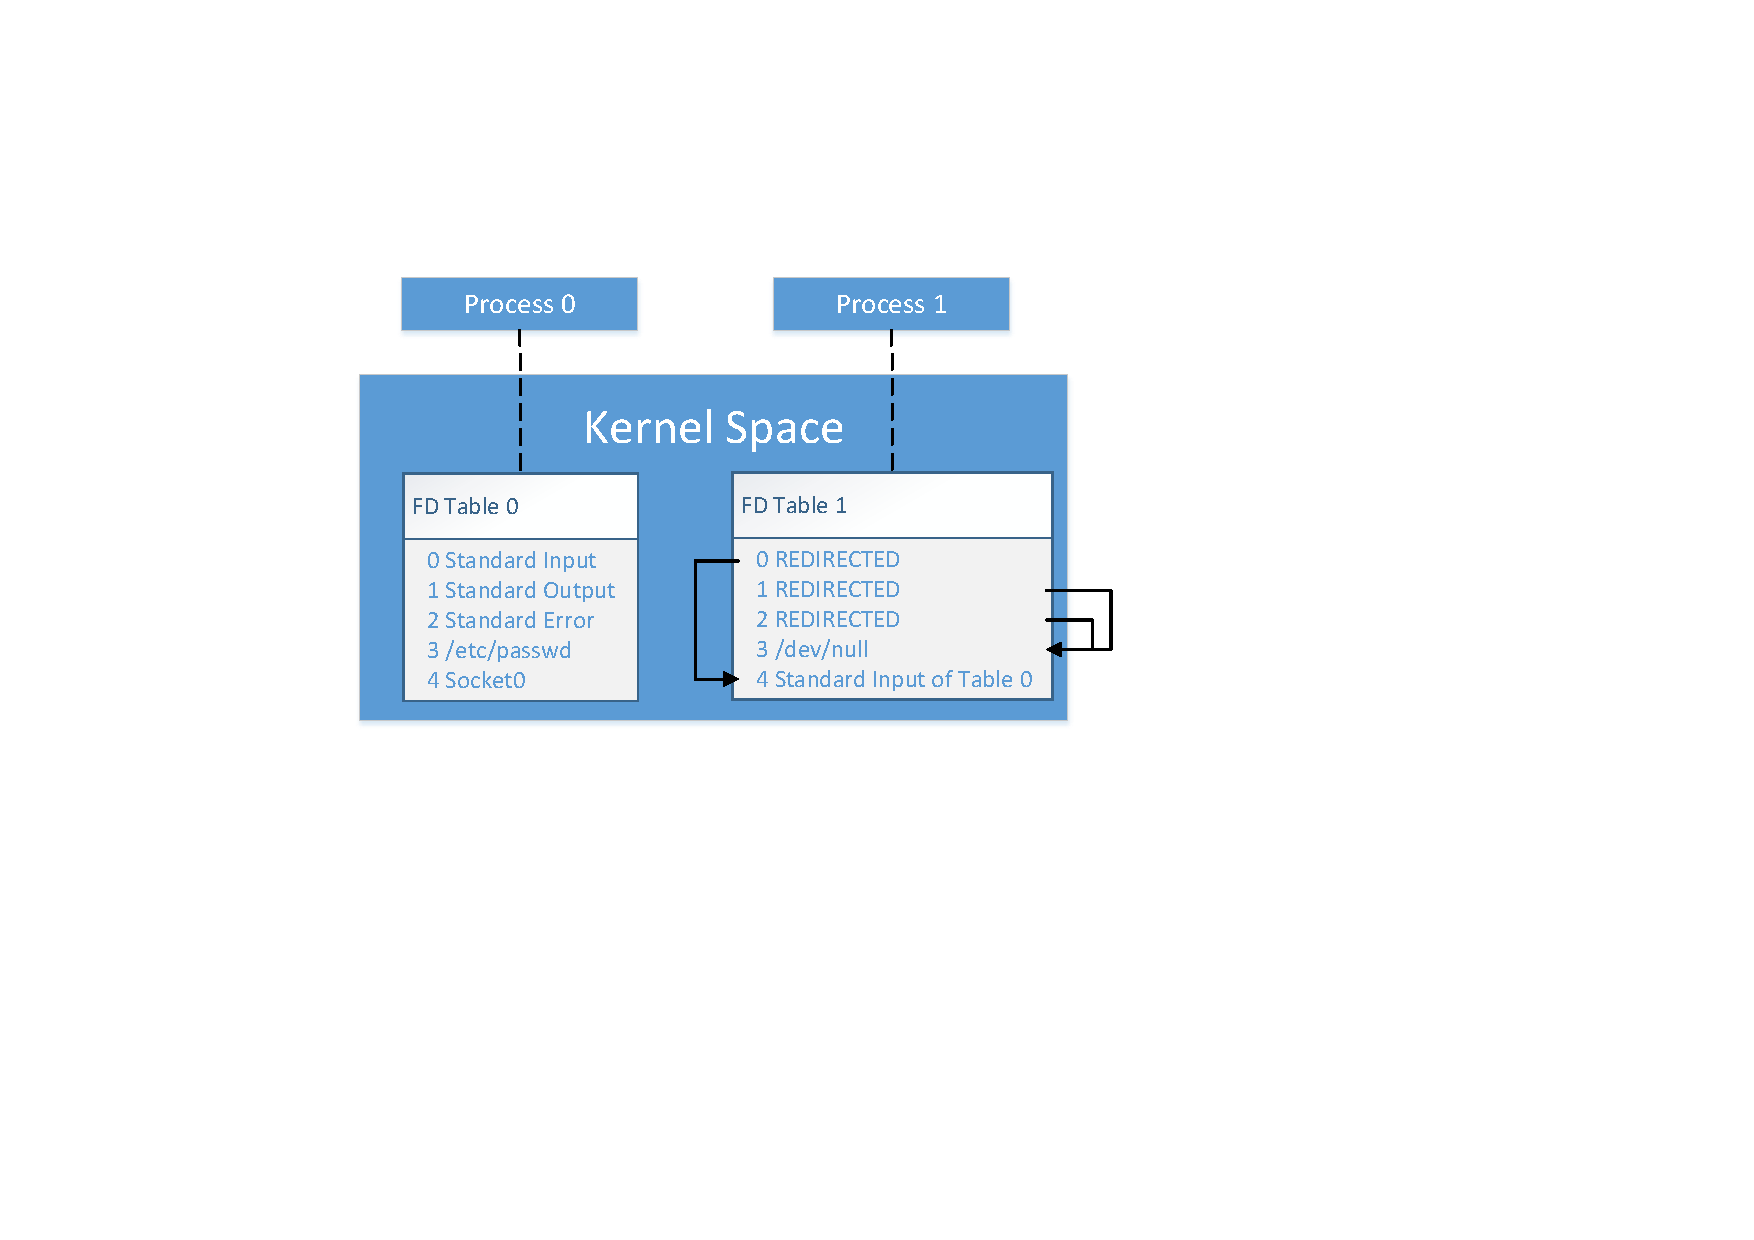
\includegraphics[width=0.6\textwidth]{\rootingFigs/file_descriptor.pdf}
  \end{center}
  \caption{File Descriptor Tables}
  \label{fig:rooting:FDTables}
\end{figure}
 

Figure~\ref{fig:rooting:FDTables} shows the file descriptor tables of two processes.
The table of Process 0 is quite simple. It has three
standard I/O FDs (indices 0, 1, 2), a file descriptor (index 3) for an opened file, and 
another file descriptor (index 4) for a socket.
Table 1 is a little bit more complicated. It opened a device named \texttt{/dev/null}, and received a 
file descriptor from Table 0, and store the descriptor at index 4. 
Moreover, Process 1's standard output and error are redirected to \texttt{/dev/null}, while its
standard input is redirected to the one (index 4) received from Process 0. 
The consequence of such redirections is that Process 1 will take exactly the same input 
as Process 0, but all outputs are abandoned~(\texttt{/dev/null} is a standard device that
functions like a black hole: nothing written to it gets out).  


\paragraph{Creating new process.}
In Unix systems, we use the \texttt{fork()} system call to create a new process. 
The \texttt{fork()} call returns an integer: for the child
process, the return value is 0, while for the parent process, the return value
is the actual process id (which is non-zero) of the newly created child process. 
The child process inherits the  parent’s data and execution status, as well as the
file descriptors. A sample code is provided in the following:

\begin{lstlisting}[frame=single, caption={}, label=label]
pid_t pid = fork();
if (pid == 0) {
    // This branch will only be executed by the child process.
    // Child process code is placed here ...
}
else {
    // This branch will only be executed by the parent process.
    // Parent process code is placed here ...
}
\end{lstlisting}
 


\begin{figure}[htb]
  \begin{center}
    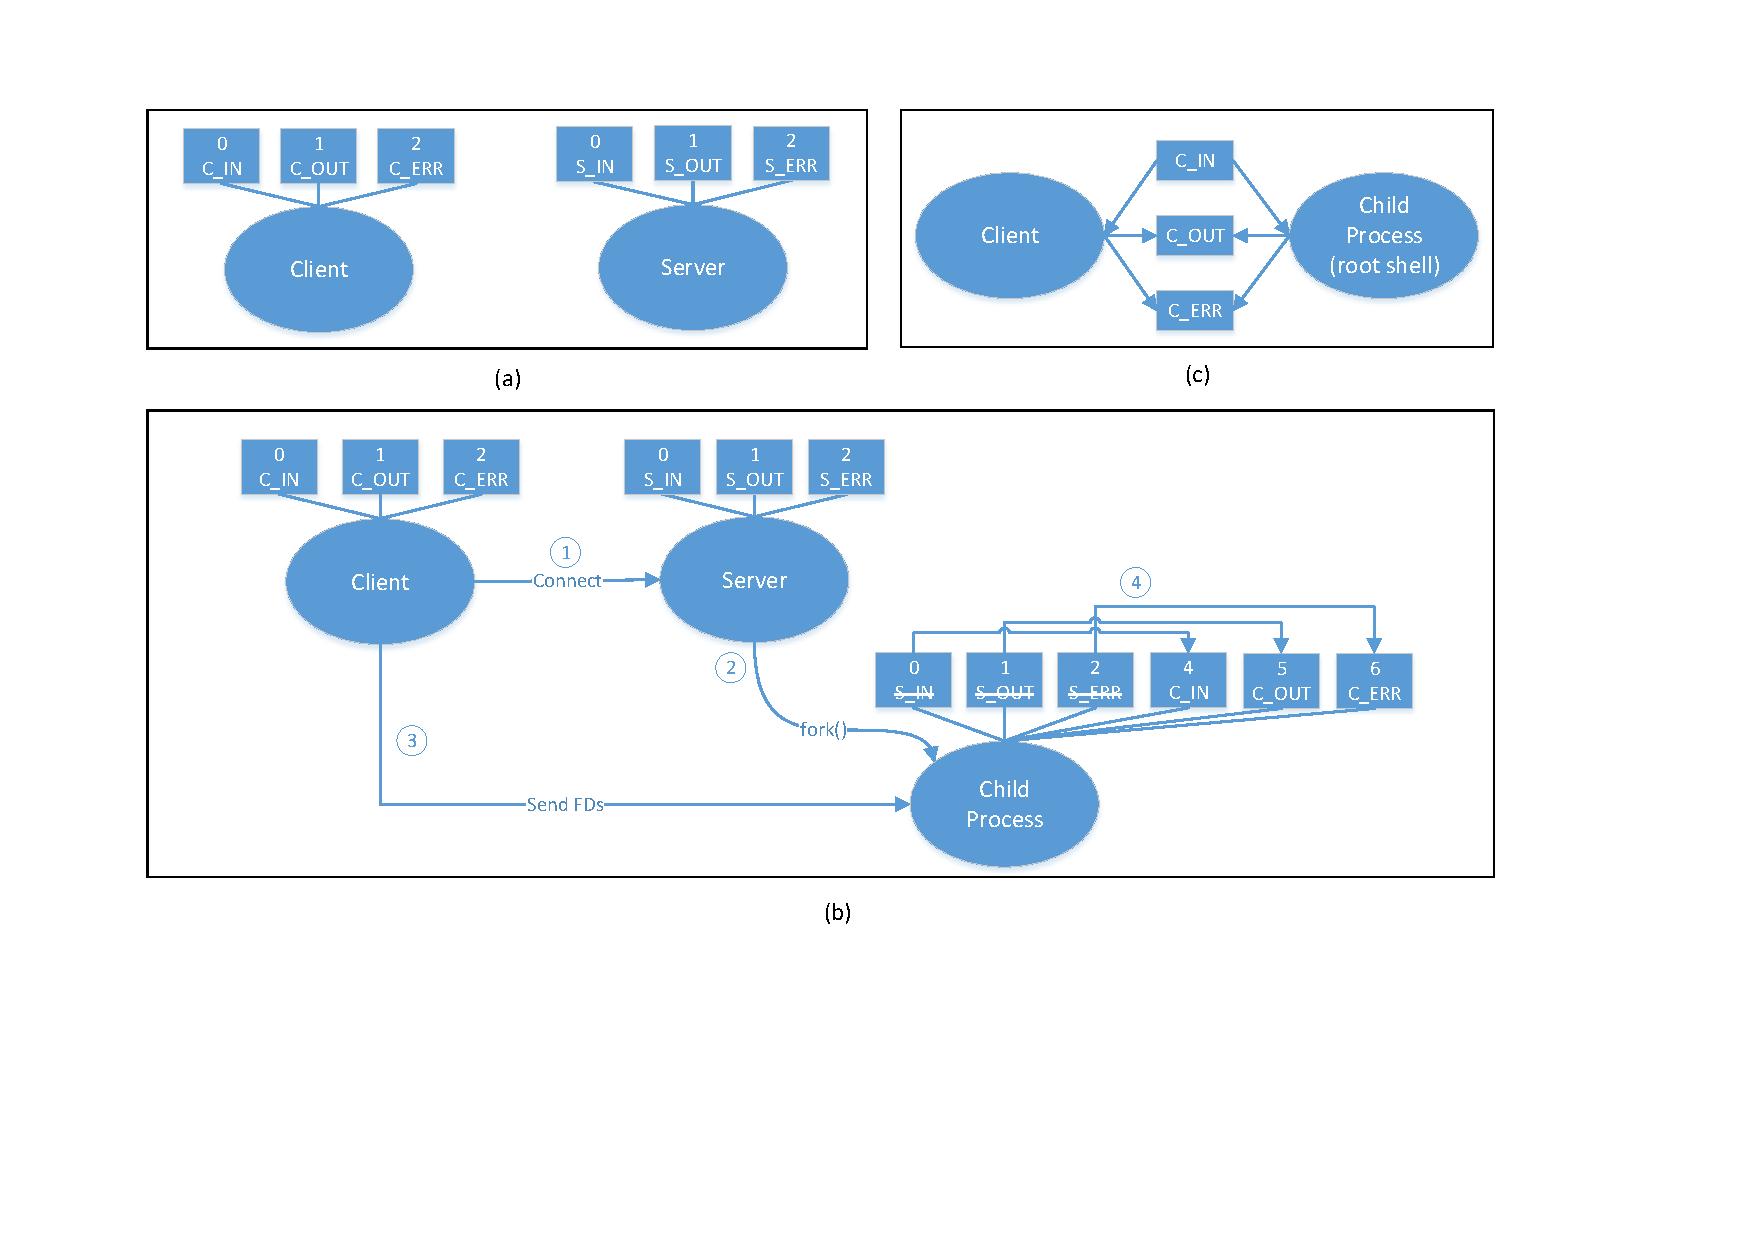
\includegraphics[width=1.0\textwidth]{\rootingFigs/dispatch_control_of_process.pdf}
  \end{center}
  \caption{How one process (Client) gains the control of the
       input/output devices of another process}
  \label{fig:rooting:dispatchingControl}
\end{figure}
 


\paragraph{Passing the File Descriptors.} 
Figure~\ref{fig:rooting:dispatchingControl} shows how to use the three standard I/O file
descriptors to help the client gain the full control of the root shell created by the server. 
Initially, as shown in Figure~\ref{fig:rooting:dispatchingControl}(a), 
the client and server are running in different processes,
while the client has a normal privilege and the server has the root
privilege. Each of them has its own standard I/O FDs 0, 1, 2. 
In the figure, the client FDs are denoted as 
\texttt{C\_IN}, \texttt{C\_OUT}, and \texttt{C\_ERR}, 
and the server’s FDs are denoted as \texttt{S\_IN}, \texttt{S\_OUT}, 
and \texttt{S\_ERR}. 
In Figure~\ref{fig:rooting:dispatchingControl}(b), we depict 
how the client and the server work together to help the client 
get the root privilege. 

\begin{enumerate}
  \item The client connects to the server using the Unix Domain Socket.

  \item Upon receiving the request, the server forks a child process and
	  runs a root shell. The child process inherits 
	  all the standard I/O FDs from the parent.

  \item The client sends its FDs 0, 1, and 2 to the server's child process using the Unix
	  Domain Socket. These FDs will be saved in 
	  the table indices 4, 5, and 6, respectively. 

  \item The child process redirects its FDs 0, 1, 2 to the FDs received
	  from the client, resulting in FDs 4, 5, and 6 being used 
	  the as the standard input, output, and error devices. Since these
	  three devices are the same as those in the client, essentially,
	  the client process and the server's child process now share the
	  same I/O devices
	  (Figure~\ref{fig:rooting:dispatchingControl}(c)). Although the
	  client process is still running with a normal user privilege, it
	  has the full control of the server's child process, which is
	  running with the root privilege.
	  
\end{enumerate}



\subsection{The Task}

Due to the complexity of the client and server program, we provide all the source code to
students from our web site. Please compile the code using NDK, and
use the method described in the previous task to build an OTA package. Students need to
demonstrate that they can successfully get the root shell after they have rooted the Android
OS using their OTA package. 


Moreover, they need to show that their client process and the shell process do share the same
standard input/output devices.  In Unix-like systems, file descriptors of a process can be found
in the \texttt{/proc} virtual file system, inside the \texttt{/proc/<PID>/fd/} folder, 
where \texttt{<PID>} is the process id. We can use the \texttt{ps} command to find out the
id of a process. 


After completing the task, students need to look at the source code, and indicate 
where the following actions occur. Filename, function name, and line number
need to be provided in the answer.

  
  \begin{itemize}
     \item Server launches the original \texttt{app\_process} binary
     \item Client sends its FDs
     \item Server forks to a child process
     \item Child process receives client's FDs
     \item Child process redirects its standard I/O FDs
     \item Child process launches a root shell
  \end{itemize}

 


\section{Guidelines}
\label{sec:rooting:guidelines}


\subsection{Android Booting Sequence and \texttt{app\_process}}
\label{sec:rooting:BootingSequence}


\begin{figure}[htb]
  \begin{center}
    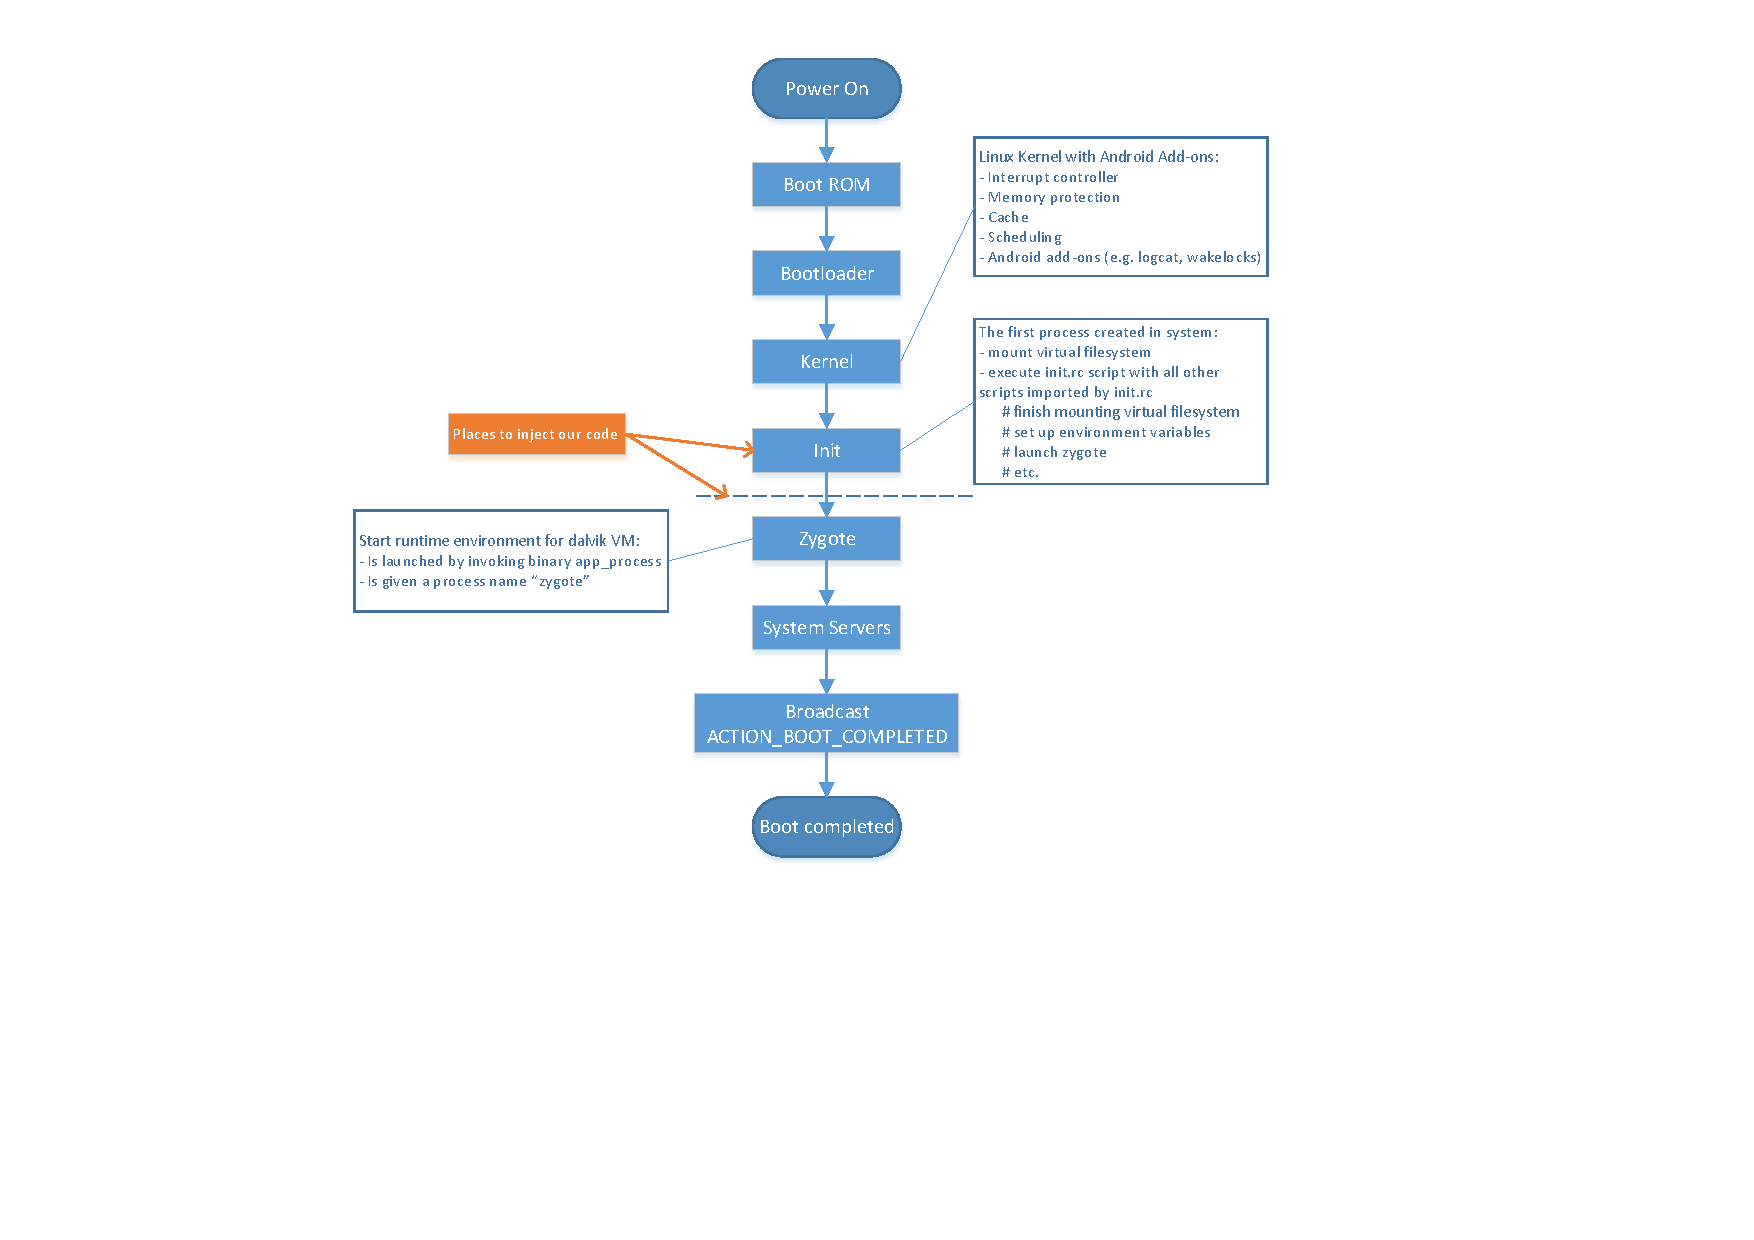
\includegraphics[width=0.8\textwidth]{\rootingFigs/full_booting_process.pdf}
  \end{center}
  \caption{Detailed Booting Process}
  \label{fig:rooting:bootingProcess}
\end{figure}

Figure~\ref{fig:rooting:bootingProcess} shows a detailed booting process. 
In the figure, we assume that the bootloader
choses to boot the Android OS, not the recovery OS.

\paragraph{Phase I: The Kernel.}
After the bootloader switches the control to Android system, Android kernel will be loaded and
starts initializing the system. Android kernel is in fact a Linux kernel, 
which handles some essential parts of the system, such as interruptions, memory protections,
scheduling etc. Some Android-specific functionalities are added to the kernel,
including logcat logger and wakelocks. 

\paragraph{Phase II: The \texttt{Init} Process.}
After the kernel is loaded, \texttt{Init} is created as the first user-space process. It is the starting
point for all other processes, and it is running under the root privilege. 
\texttt{Init} initializes the virtual file system, detects hardware, 
then executes script file \texttt{init.rc} to configure the system.
The script \texttt{init.rc} itself mainly focuses on mounting files inside virtual file system and
initializes system daemons. However, it imports some other \texttt{rc} script files for various
purposes, such as setting up environment variables, executing architecture specific commands,
and launching \texttt{zygote}. Here are the files imported to \texttt{init.rc}: 

\begin{itemize}
  \item \texttt{init.environ.rc}: Environment variables are set by \texttt{init.environ.rc},
    which provides some important path-related environment variables.  These paths are very
    important for launching further processes because many of them will try to access these
    paths using the corresponding environment variable names. In one
    of the lab tasks, we need to pass environment variables to the child process; now we see
    why that is needed.  

  \item \texttt{init.\$\{ro.hardware\}.rc}: Some commands or codes are architecture specific.
    The variable \texttt{\$\{ro.hardware\}} is inherited from the \texttt{Init} process and passed to 
    the \texttt{init.rc} script. On our Android-x86 VM, it will be ``android\_x86'' and the
    script file \texttt{init.android\_x86.rc} file will be invoked. 
    Inside this file, \texttt{init.sh} is called. This \texttt{init.sh} file
    is the one used in In Task 1, where we inject the invocation of our code.

  \item \texttt{init.\$\{ro.zygote\}.rc}: This file starts a very important daemon called
    \texttt{Zygote}.  The variable \texttt{\$\{ro.zygote\}} is inherited
    from the \texttt{Init} binary. It can be \texttt{zygote32} or \texttt{zygote64}, for 32-bit
    and 64-bit architecture, respectively; it can also be \texttt{ zygote32\_64} or \texttt{zygote64\_32} 
    for hybrid modes (mainMode\_secondaryMode).  In our Android-x86 VM, 
    it is \texttt{init.zygote32.rc}.  
    
    
\end{itemize}


All these \texttt{rc} script files are stored in an image file, named \texttt{ramdisk.img}
on our Android-x86 VM; on real devices, these script files are inside \texttt{boot.img}, 
which contains \texttt{ramdisk.img} and the kernel.
The \texttt{ramdisk.img} file will be extracted into the memory while booting
up. Making modifications directly on an image file is not very easy. That is the main reason
why we only change the \texttt{init.sh} file in our first task, because  
the \texttt{init.sh} file is inside the \texttt{/system} folder, not inside 
those image files. 


\paragraph{Phase III: The \texttt{Zygote} Process.}
In the \texttt{init.\$\{ro.zygote\}.rc} file, a special daemon is launched by the \texttt{Init}
process via the \texttt{"service zygote /system/bin/app\_process ..."} command (options are
omitted). The command starts a daemon called \texttt{zygote}, which executes 
the \texttt{app\_process} binary.
Zygote is the starting point of the Android runtime.
It starts the runtime environment of Dalvik or ART, which are virtual machines that run Java programs. 
In Android, system servers and most applications are written in Java, so \texttt{Zygote} is
an essential daemon, and it runs with the root privilege. 

That makes \texttt{app\_process} another place to insert our rooting code. 
The \texttt{app\_process} file is not a real binary file; it is a symbolic link, pointing to
either \texttt{app\_process32} or \texttt{app\_process64}, depending on the architecture of the system. 
Therefore, we just need to change the symbolic link, and let it point to our code. 
In our code, we will have two processes, one running our rooting code, and the other running 
the original \texttt{app\_process} code.  
This approach is commonly used by many existing rooting OTA packages. 



\subsection{How to unlock the boot loader on a real device}

As what is shown in Figure~\ref{fig:rooting:bootingProcess}, when the power
button is pressed, the device firsts goes to a fixed location in its ROM, and run
instructions from there. These instructions will then 
go to a pre-defined location on the disk or flash drive to 
load the bootloader, and pass the control to it. 
Bootloader then loads the operating system, and eventually gives the control
to the loaded OS.


Most of the Android devices come with two operating systems, an Android OS
and a recovery OS. By default, the bootloader will choose the Android OS to 
boot; however, if some special key combination is pressed during the
booting, the bootloader will boot the recover OS instead. On Nexus devices,
this is achieved by pressing the ``Volume Down'' and ``Power'' buttons together.


Bootloader usually have another functionality that is often disabled by
default. This functionality allows users to replace (often called
\textit{flash}) the OS images on any of
the partitions, so users can install a different recovery OS or Android OS. 
Most manufacturers do not want users to make such kind of modifications to
their devices, so before shipping devices to customers, they 
disable the functionality, and hence we say
that ``the bootloader is locked''.  With a locked bootloader, any attempt
to flash the installed OS will be denied by the bootloader. 
The following command tries to flash the recovery OS with a locked
bootloader; as we can see, we get an error message:

\begin{lstlisting}[frame=single, caption={}, label=label]
# fastboot flash recovery CustomRecoveryOS.img
sending 'recovery' (11600 KB) ...
OKAY [ 0.483s]
writing 'recovery' ...
FAILED (remote: not supported in locked device)
finished. total time: 0.585s
\end{lstlisting}


Some vendors choose to permanently lock the bootloader; in this case, it
will be very hard to flash the OSes on the devices. However,  
many vendors choose not to do so, and instead, they 
provide instructions to unlock the bootloader, so users who really want to
flash their devices can still do that. We will show how to unlock the
bootloader. For the demonstration purpose we are using a Nexus device.
To unlock it, first we need to load
bootloader of the Nexus device by passing the \texttt{"adb reboot
bootloader"} command or by interrupting the normal boot process using 
the ``volume down'' and ``power'' button combination.
Figure~\ref{fig:rooting:bootloader}(a)  shows the bootloader screen of
a Nexus 5 device, which indicates that the bootloader is
locked.

\begin{figure}[htb]
	\begin{center}
		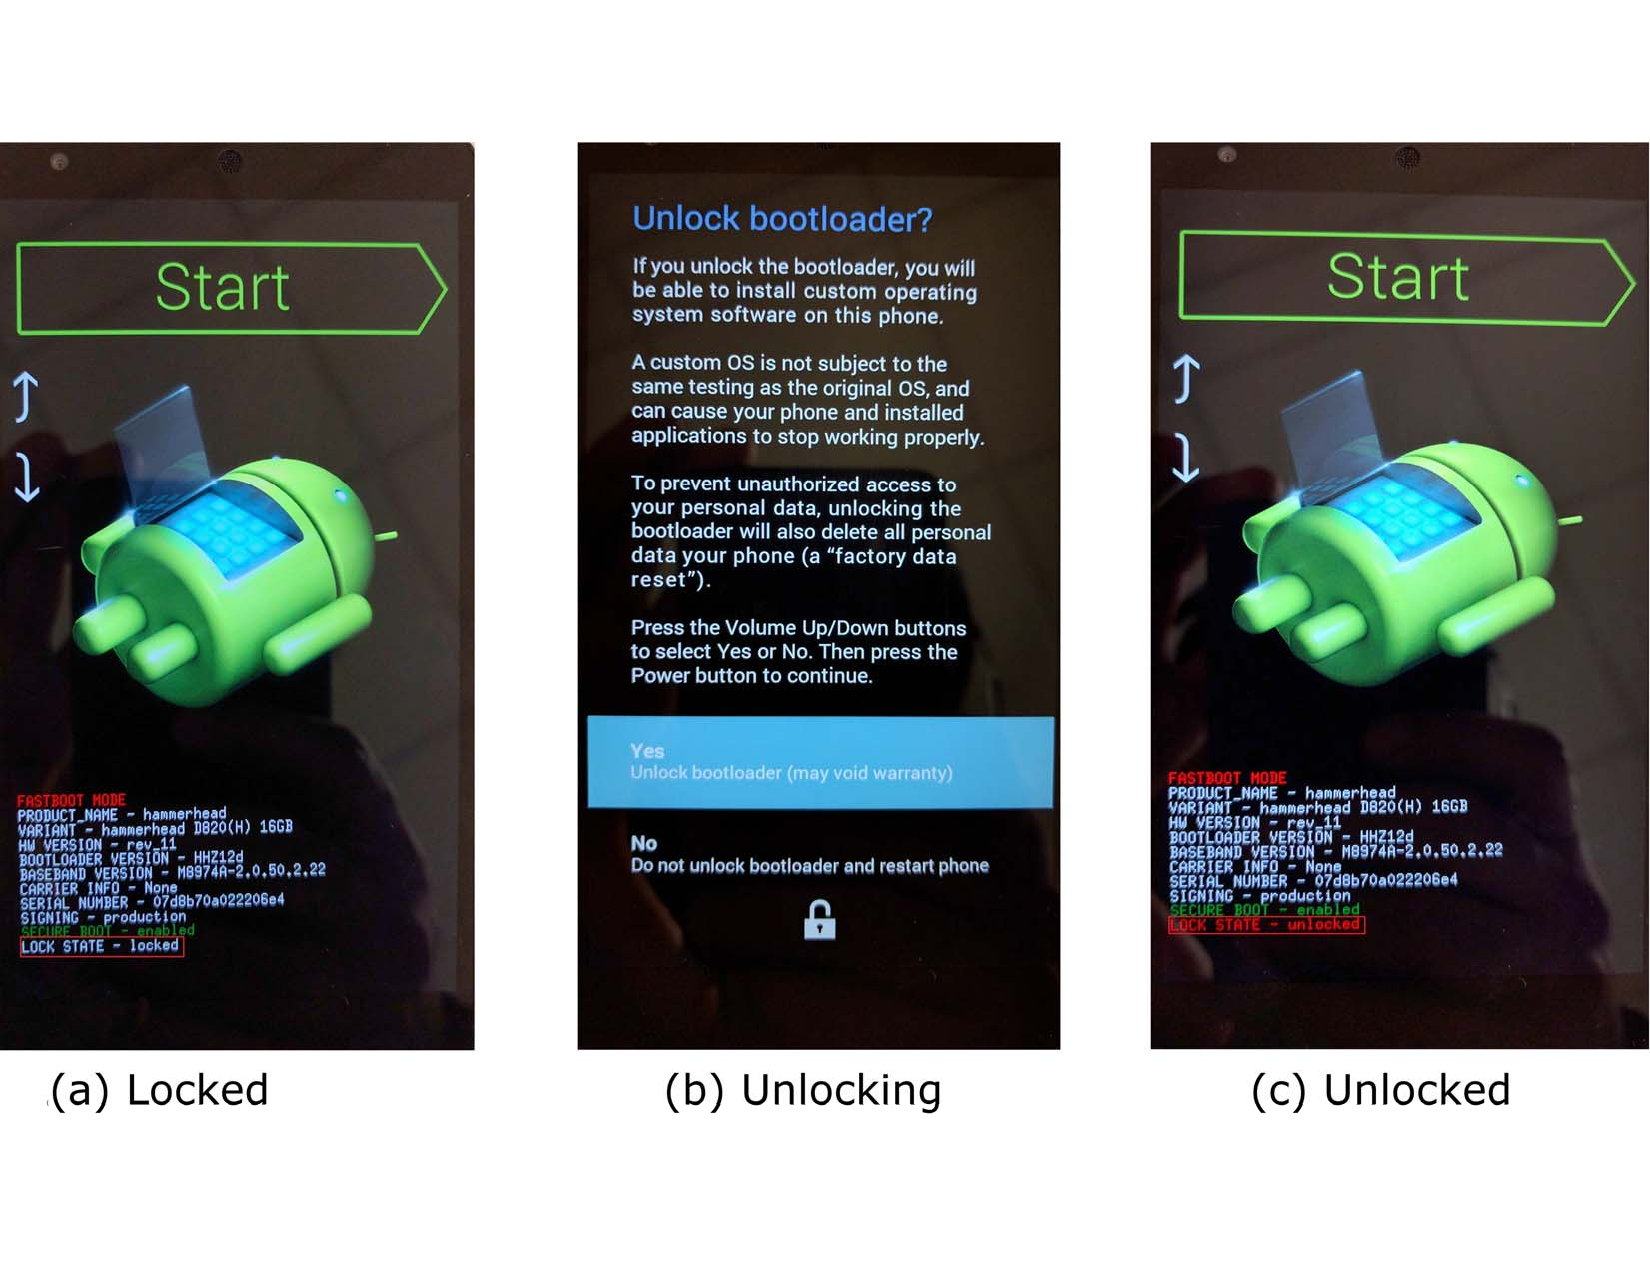
\includegraphics[width=1.0\textwidth]{\rootingFigs/Bootloader.pdf}
	\end{center}
	\caption{Unlock Bootloader}
	\label{fig:rooting:bootloader}
\end{figure}


Bootloader of Nexus devices can be unlocked by using the 
\texttt{"fastboot oem unlock"} command. 
Be very careful while unlocking the bootloader because it
will void the manufacturer's warranty and completely wipe out 
personal data on the device. We advise you to backup your personal data before
unlocking the bootloader. You can also backup your installed apps
and app data by using the \texttt{"adb backup -apk -all -f backup.ab"}
command, which creates a file called \texttt{backup.ab}. 
After unlocking the bootloader, you can restore the data by running 
\texttt{"adb restore backup.ab"}. 
Figure~\ref{fig:rooting:bootloader}(b) shows the confirmation screen, and 
Figure~\ref{fig:rooting:bootloader}(c) shows that the bootloader is now
unlocked. 




% -------------------------------------------
% SUBSECTION
% ------------------------------------------- 
\subsection{How to replace the existing recovery OS on a real device}


\begin{figure}[htb]
	\begin{center}
		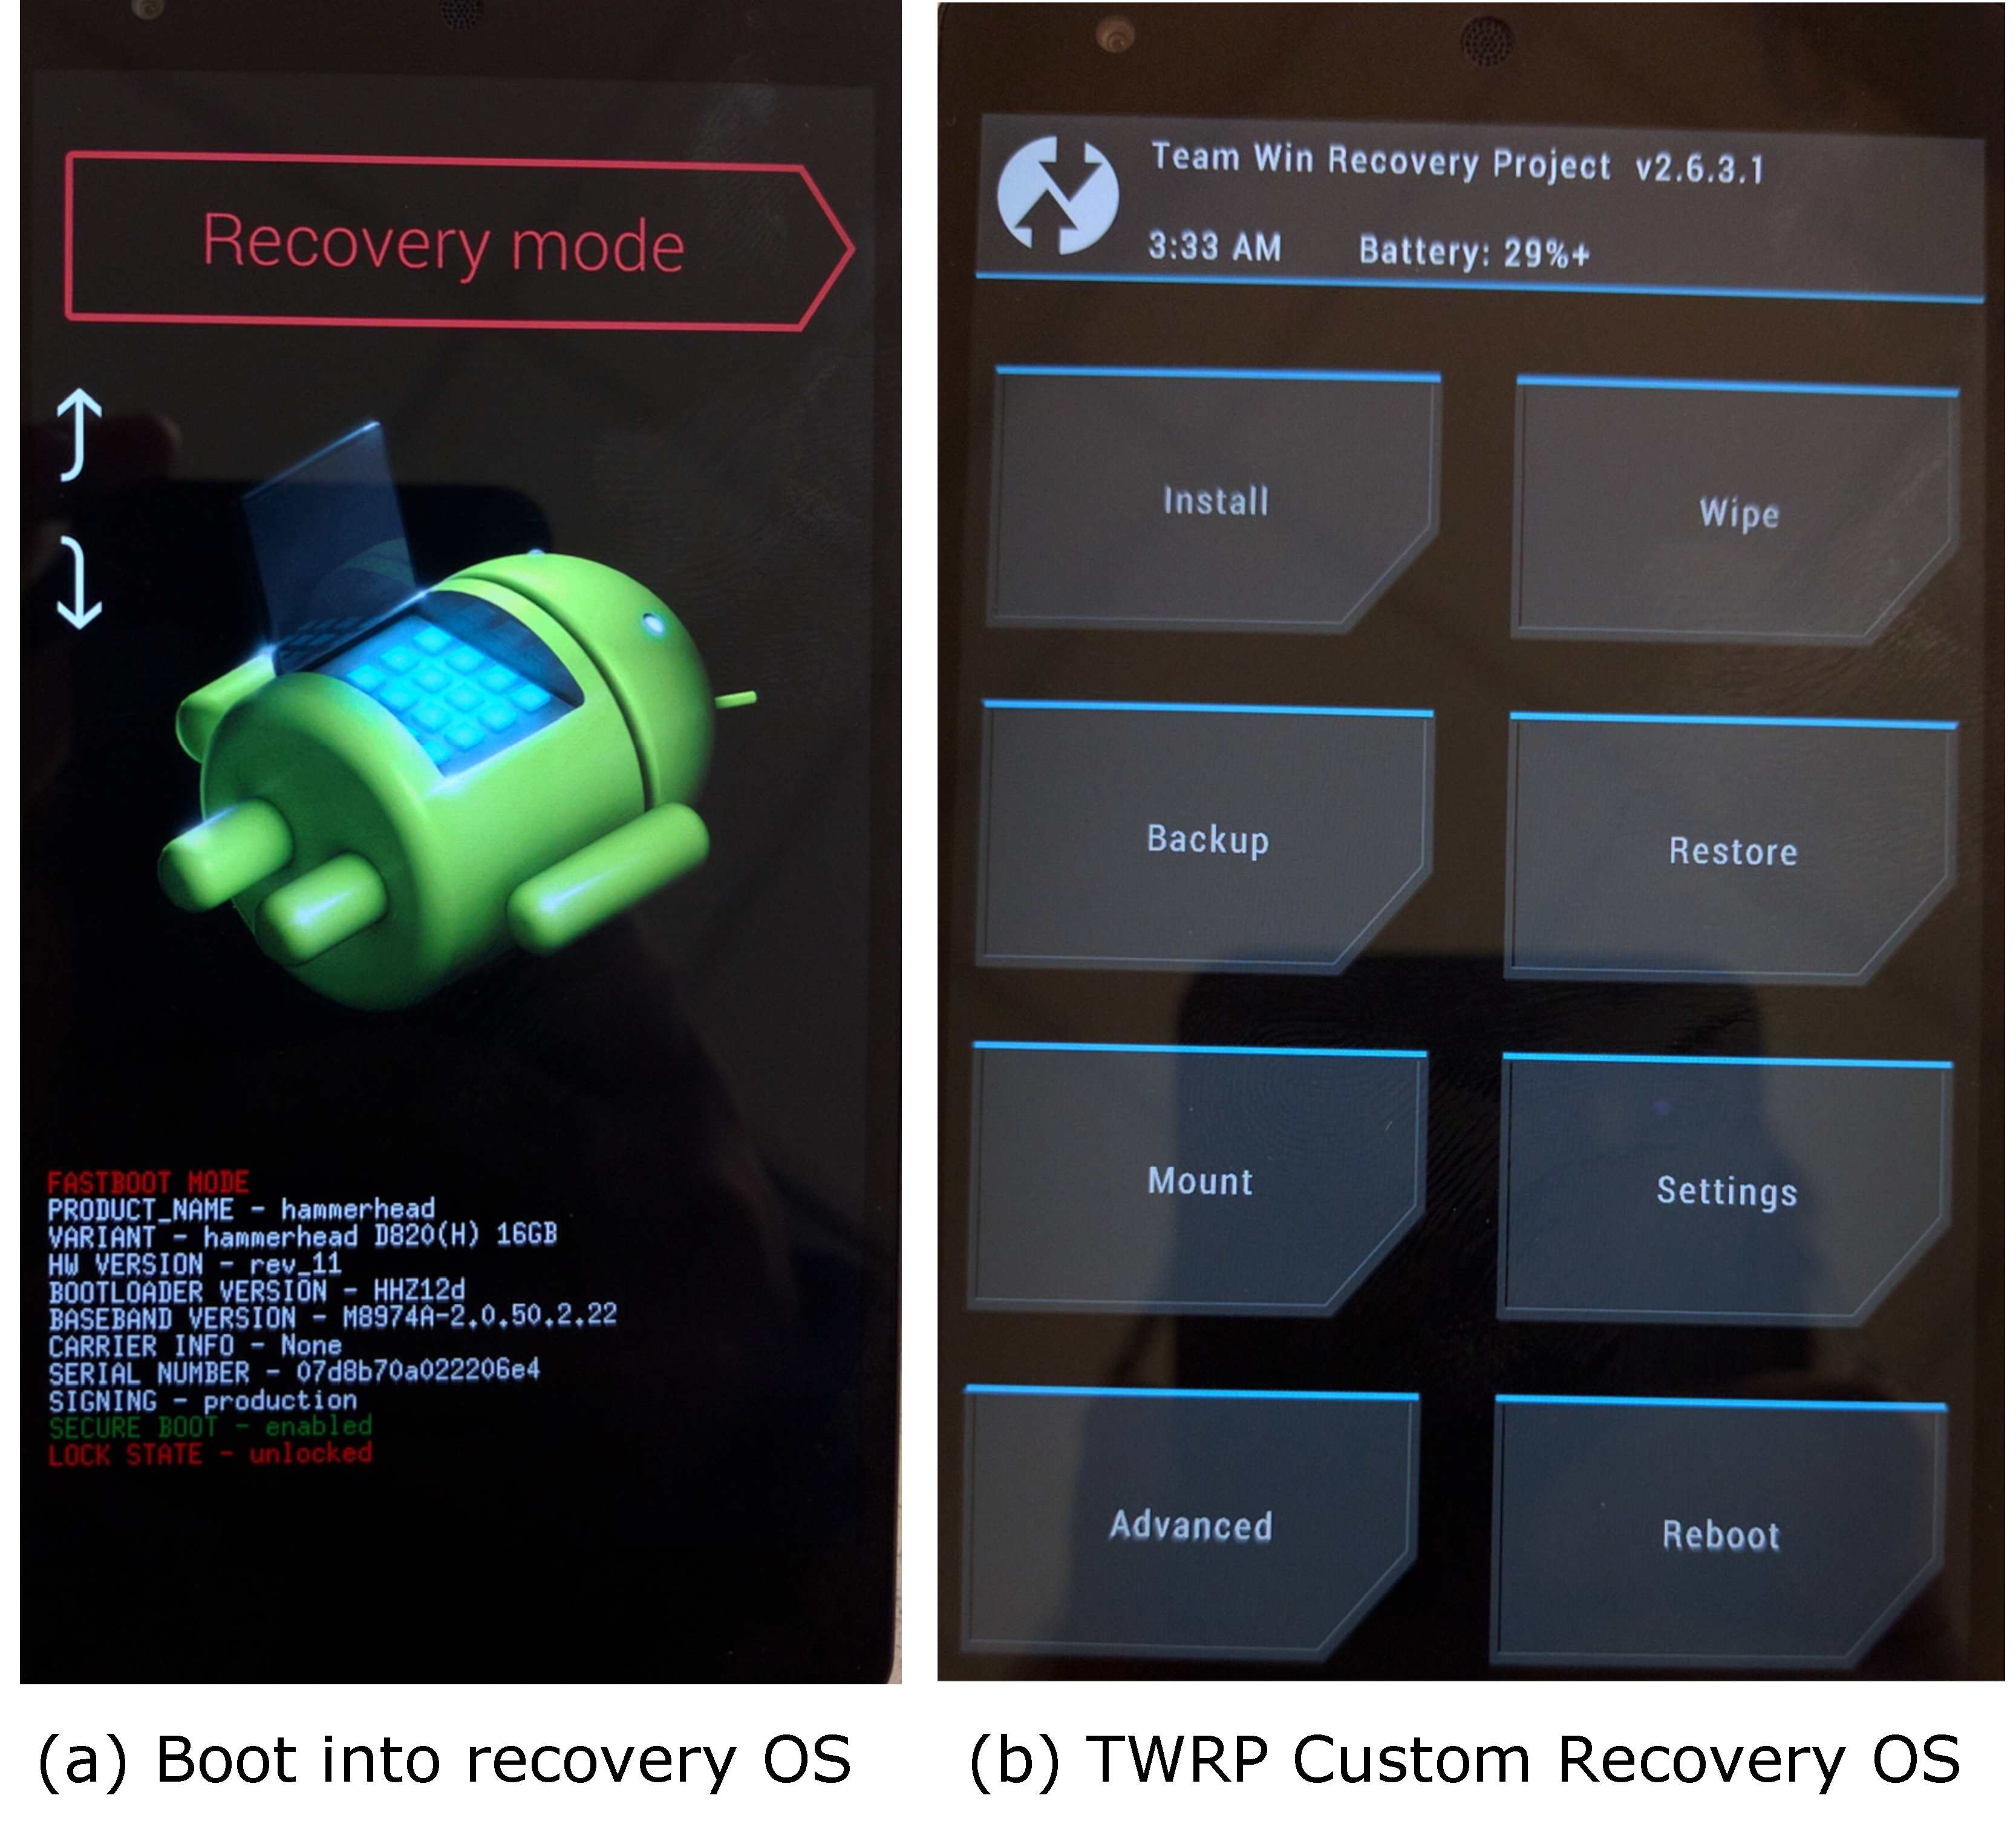
\includegraphics[width=0.6\textwidth]{\rootingFigs/RecoveryMode.pdf}
	\end{center}
	\caption{Custom Recovery OS}
	\label{fig:root:customRecoveryMode}
\end{figure}
 

On real devices, to remove the restrictions imposed by the stock
recovery OS, such as signature verification, we have to replace it with 
a custom recovery OS that does not impose such restrictions. 
A number of custom recovery OSes are available on the market. TWRP and
ClockworkMod are two of the best choices. 
We are going to use TWRP in our description. 
To flash custom recovery we need to unlock the
bootloader of the device. We assume that you have already unlocked the
bootloader. We can boot the custom Recovery OS by using
the \texttt{"fastboot boot CustomRecoveryOS.img"} command, or we can
permanently replace the device's stock recovery OS with TWRP. The following 
command flashing the custom recovery OS onto the recovery partition:


\begin{lstlisting}[frame=single, caption={}, label=label]
# fastboot flash recovery CustomRecoveryOS.img
sending 'recovery' (11600 KB) ...
OKAY [ 0.483s]
writing 'recovery' ...
OKAY [ 0.948s]
finished. total time: 1.435s
\end{lstlisting}

After that, we can boot into the recovery OS by 
pressing the ``volume down'' and ``power'' button combination during the boot-up process. 
Figure~\ref{fig:root:customRecoveryMode}(a) shows how to boot into the recovery OS, and 
Figure~\ref{fig:root:customRecoveryMode}(b) shows the user interface of the TWRP recovery OS.
As you can see, it has several useful features. 



\section{Submission and Demonstration}

You need to submit a detailed lab report to describe what you have done and
what you have observed, including screenshots and code snippets (if
needed). You also need to provide explanation to the observations that are
interesting or surprising. You are encouraged to pursue further
investigation, beyond what is required by the lab description.


\end{document}

